\documentclass{standalone}
\usepackage{tikz}
\usepackage{verbatim}
\begin{document}
\pagestyle{empty}
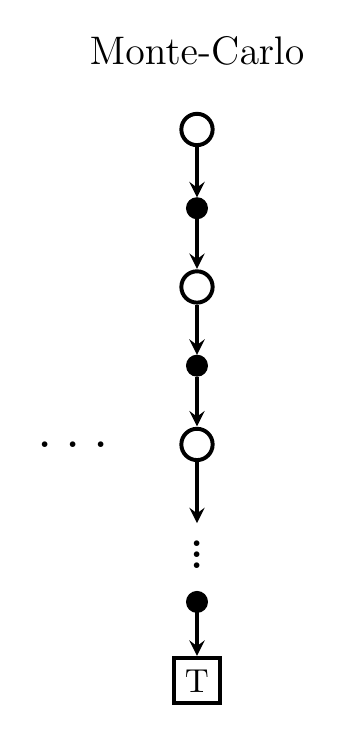
\begin{tikzpicture}

    % TD n step
  \node at (12, 1) {\Large Monte-Carlo};
  \node[draw,circle,scale=1.2, fill=white, line width=0.5mm] (s_12) at (12,0) {};
  \foreach \xa in {-1,-3} {
      \node[draw,circle,fill,scale=0.8] (b12\xa) at (12, \xa) {};
      \node[draw,circle,scale=1.2, fill=white,line width=0.5mm] (s12\xa) at (12,\xa-1) {};
      \draw[-stealth, line width=0.5mm] (b12\xa) -- (s12\xa);
  }
  \draw[-stealth, line width=0.5mm] (s_12) -- (b12-1);
  \draw[-stealth, line width=0.5mm] (s12-1) -- (b12-3);
  \draw[-stealth, line width=0.5mm] (s12-3) -- (12,-5);
  \node[draw,circle,fill,scale=0.8] at (12, -6) {};
  \node[draw,rectangle, scale=1.2, line width=0.5mm] (s12b) at (12, -7) {T};
  \node at (12, -5.3) {\Huge \vdots};
  \node at (10.5, -4) {\Huge \dots};
  \draw[-stealth, line width=0.5mm] (12,-6) -- (s12b);

\end{tikzpicture}
\end{document}